\section{Modello Computazionale}
%%%%%%%%%%%%%%%%%%%%%%%%%%%%%%%%%%%%%%%%%%%%%%%%%%%%%%%%%%%%%%%%%%%%%%%%%%%%%%%%
%%%%%%%%%%%%%%%%%%%%%%%%%%%%%%%%%%%%%%%%%%%%%%%%%%%%%%%%%%%%%%%%%%%%%%%%%%%%%%%%
\begin{frame}
\frametitle{Modello Computazionale}
\begin{center}
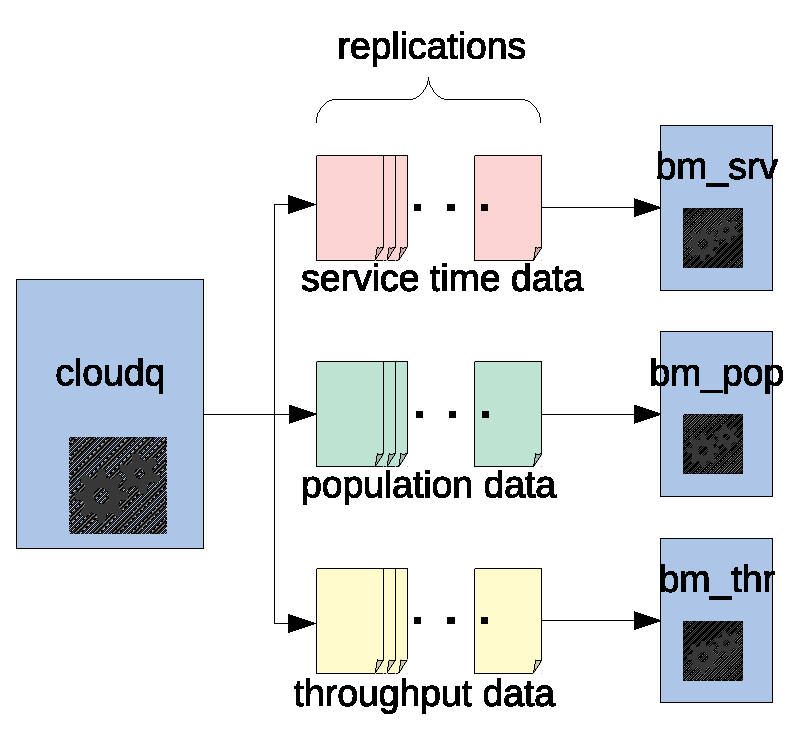
\includegraphics[width=.7\textwidth]{../figures/comp}
\end{center}
\end{frame}
%%%%%%%%%%%%%%%%%%%%%%%%%%%%%%%%%%%%%%%%%%%%%%%%%%%%%%%%%%%%%%%%%%%%%%%%%%%%%%%%
%%%%%%%%%%%%%%%%%%%%%%%%%%%%%%%%%%%%%%%%%%%%%%%%%%%%%%%%%%%%%%%%%%%%%%%%%%%%%%%%
\begin{frame}[fragile]
\frametitle{Modello Computazionale: Next Event Simulation}
\begin{columns}
\column{.5\textwidth}
\begin{lstlisting}
typedef struct {     
    double current;  
    double next;     
} clock;

struct job_t {
    unsigned long id;
    unsigned int class;
    unsigned int node;
    double service[5];
};

struct event {
    double time;
    struct job_t job;
    unsigned int type;
};
\end{lstlisting}
\column{.5\textwidth}
\begin{itemize}
\item prossimo arrivo di un job
\item al più $N$ completamenti di job nel cloudlet
\item $0$ o più completamenti di job nel cloud
\item $0$ o più completamenti di fase di setup dei job interrotti
\end{itemize}
~

\includegraphics[width=\textwidth]{../figures/eventq}
\end{columns}
\end{frame}
%%%%%%%%%%%%%%%%%%%%%%%%%%%%%%%%%%%%%%%%%%%%%%%%%%%%%%%%%%%%%%%%%%%%%%%%%%%%%%%%
%%%%%%%%%%%%%%%%%%%%%%%%%%%%%%%%%%%%%%%%%%%%%%%%%%%%%%%%%%%%%%%%%%%%%%%%%%%%%%%%
\begin{frame}[fragile]
\frametitle{Modello Computazionale: Flusso principale}
\begin{columns}
\column{.5\textwidth}
\begin{lstlisting}
/* initialize data structures */
/* ..... */

while (queue.head != NULL) { 

    e = dequeue_event(&queue);
    t.next = e->time;

    for (i = 0; i < 5; i++)
        area[i] += (t.next - t.current) * n[i];

    t.current = t.next;   

    switch (e->type) {
    case E_ARRIVL:              
        /* process an arrival */
        /* ..... */
    case E_SETUP:
        /* process an setup phase */
        /* ..... */
    case E_DEPART: 
        /* process a departure */
        /* ..... */
        /* write data to outfile */
        /* ..... */
    default:
        handle_error("unknown event type");
    }
}

/* ..... */
\end{lstlisting}
\column{.5\textwidth}
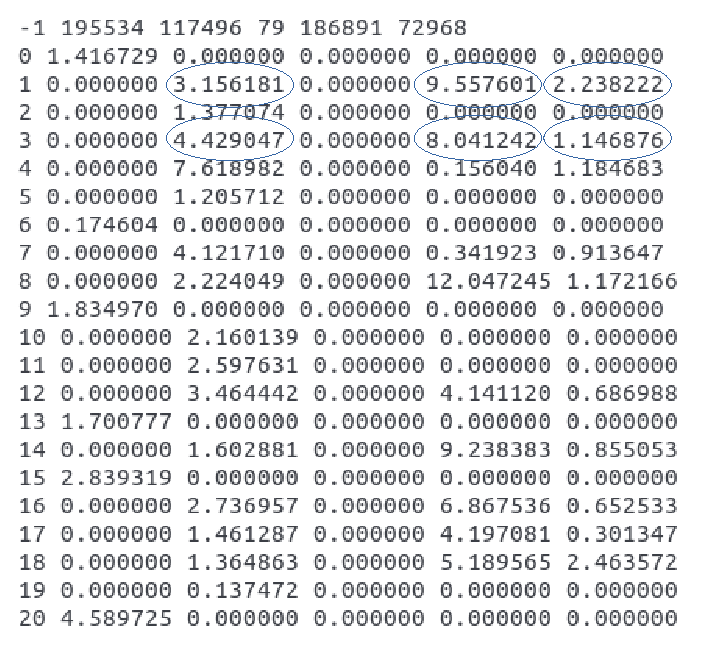
\includegraphics[width=\textwidth]{../figures/srvdat}
\end{columns}
\end{frame}

%%%%%%%%%%%%%%%%%%%%%%%%%%%%%%%%%%%%%%%%%%%%%%%%%%%%%%%%%%%%%%%%%%%%%%%%%%%%%%%%
%%%%%%%%%%%%%%%%%%%%%%%%%%%%%%%%%%%%%%%%%%%%%%%%%%%%%%%%%%%%%%%%%%%%%%%%%%%%%%%%
\begin{frame}[fragile]
\frametitle{Modello Computazionale: Batch Means}
\begin{lstlisting}
// compute batch sizes
b = (c1_clet + c2_clet + c1_cloud + c2_cloud) / K;
b1 = (c1_clet + c1_cloud) / K;
b2 = (c2_clet + c2_cloud) / K;
b_clet = (c1_clet + c2_clet) / K;
b1_clet = c1_clet / K;
b2_clet = c2_clet / K;
b_cloud = (c1_cloud + c2_cloud) / K;
b1_cloud = c1_cloud / K;
b2_cloud = c2_cloud / K;
b_intr = c_setup / K;

// get data
while (fscanf(file, "%ld %lf %lf %lf %lf %lf\n", &id,
        &s1_clet, &s2_clet, &s1_cloud, &s2_cloud, &setup) != EOF) {

    s[id / b] += s1_clet + s2_clet + s1_cloud + s2_cloud + setup;

    if (s1_clet || s1_cloud) {
        s1[n1 / b1] += s1_clet + s1_cloud;
        n1++;
    }
    if (s2_clet || s2_cloud) {
        s2[n2 / b2] += s2_clet + s2_cloud + setup;
        n2++;
    }
    if (s1_clet) {
        s1clet[n1_clet / b1_clet] += s1_clet;
        sclet[(n1_clet + n2_clet) / b_clet] += s1_clet;
        n1_clet++;
    }
\end{lstlisting}
\end{frame}
\begin{frame}[fragile]
\frametitle{Modello Computazionale: Batch Means}
\begin{lstlisting}
    if (s2_clet && !setup) {
        s2clet[n2_clet / b2_clet] += s2_clet;
        sclet[(n1_clet + n2_clet) / b_clet] += s2_clet;
        n2_clet++;
    }
    if (s1_cloud) {
        s1cloud[n1_cloud / b1_cloud] += s1_cloud;
        scloud[(n1_cloud + n2_cloud) / b_cloud] += s1_cloud;
        n1_cloud++;
    }
    if (s2_cloud) {
        s2cloud[n2_cloud / b2_cloud] += s2_cloud;
        scloud[(n1_cloud + n2_cloud) / b_cloud] += s2_cloud;
        n2_cloud++;
    }
    if (setup) {
        sintr[n_intr / b_intr] += s2_clet + s2_cloud + setup;
        n_intr++;
    }
}
// compute batch means
for (i = 0; i < K; i++) {
    s[i] /= b;
    s1[i] /= b1;
    s2[i] /= b2;
    s1clet[i] /= b1_clet;
    s2clet[i] /= b2_clet;
    sclet[i] /= b_clet;
    s1cloud[i] /= b1_cloud;
    s2cloud[i] /= b2_cloud;
    scloud[i] /= b_cloud;
    sintr[i] /= b_intr;
}
\end{lstlisting}
\end{frame}
%%%%%%%%%%%%%%%%%%%%%%%%%%%%%%%%%%%%%%%%%%%%%%%%%%%%%%%%%%%%%%%%%%%%%%%%%%%%%%%%
%%%%%%%%%%%%%%%%%%%%%%%%%%%%%%%%%%%%%%%%%%%%%%%%%%%%%%%%%%%%%%%%%%%%%%%%%%%%%%%%
